\documentclass[usenames,dvipsnames]{beamer}
\usepackage[utf8]{inputenc}
\usepackage[T1]{fontenc}
\usepackage[french]{babel}
\usepackage{xcolor}
\usepackage{pifont}
\usepackage{float}
\usetheme{Singapore} %Boadilla | Bergen | Madrid | Antibes | Hannover | Singapore | Warsaw

\newcommand{\cmark}{\ding{51}}
\newcommand{\xmark}{\ding{55}}
%----------------------------------------------------------------------------------------
%   TITLE INFORMATION
%----------------------------------------------------------------------------------------
\title{Classification de données textuelles}
\subtitle{HMIN232M -- Méthodes de la science des données}
\author{B. Rima \and E. Youssef \and T. Shaqura}
\institute[UM]{M1 Informatique AIGLE}
\date{28 avril 2019}

\begin{document}
%----------------------------------------------------------------------------------------
%   TITLE FRAME
%----------------------------------------------------------------------------------------
\begin{frame}
\titlepage
\end{frame}
%----------------------------------------------------------------------------------------
%   OUTLINE
%----------------------------------------------------------------------------------------
\begin{frame}{Sommaire}
\tableofcontents
\end{frame}
%----------------------------------------------------------------------------------------
%   INTRODUCTION
%----------------------------------------------------------------------------------------
\section{Visualisation des données}
\subsection{WordCloud}
\begin{frame}{WordCloud}{Visualisation des données}
\begin{columns}
\column{0.5\textwidth}
\begin{figure}
    \centering
    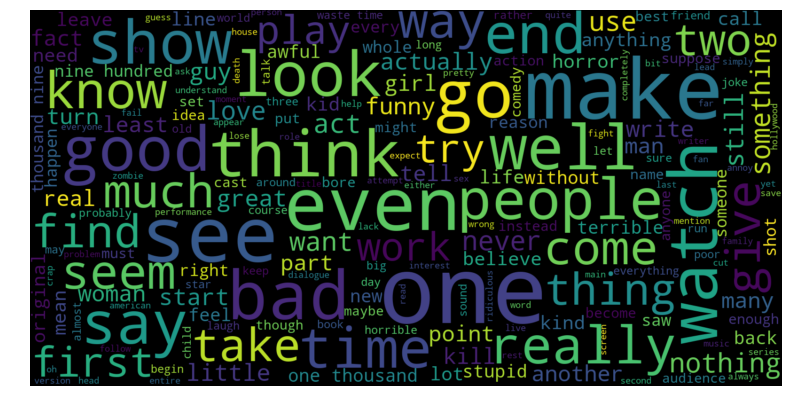
\includegraphics[width=1.0\textwidth]{images/negative_opinions_frequent_words.png}
    \caption{Mots les plus fréquents dans les avis négatifs}
    \label{fig:most_freq_neg}
\end{figure}
\column{0.5\textwidth}
On peut s'attendre à...
\begin{itemize}
    \item Beaucoup d'ironies
    \item Phrases à polarités différentes dans les avis
\end{itemize}
\end{columns}
\end{frame}

\section{Extraction des features}
\subsection{Vectorisation et sélection des features}
\begin{frame}{Vectorisation et sélection des features}{Extraction des features}
\begin{figure}
    \centering
    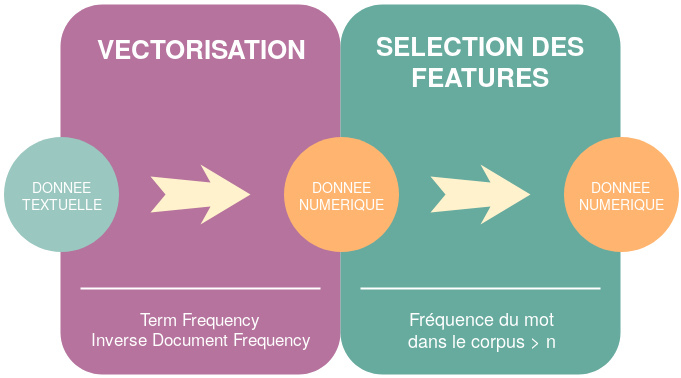
\includegraphics[scale=0.3]{images/features.png}
    \caption{Traitement des features}
    \label{fig:features}
\end{figure}
\end{frame}

\section{Pour résumer...}
\subsection{Schéma globale de nos traitements}
\begin{frame}{Schéma globale de nos traitements}{Pour résumer...}
\begin{figure}
    \centering
    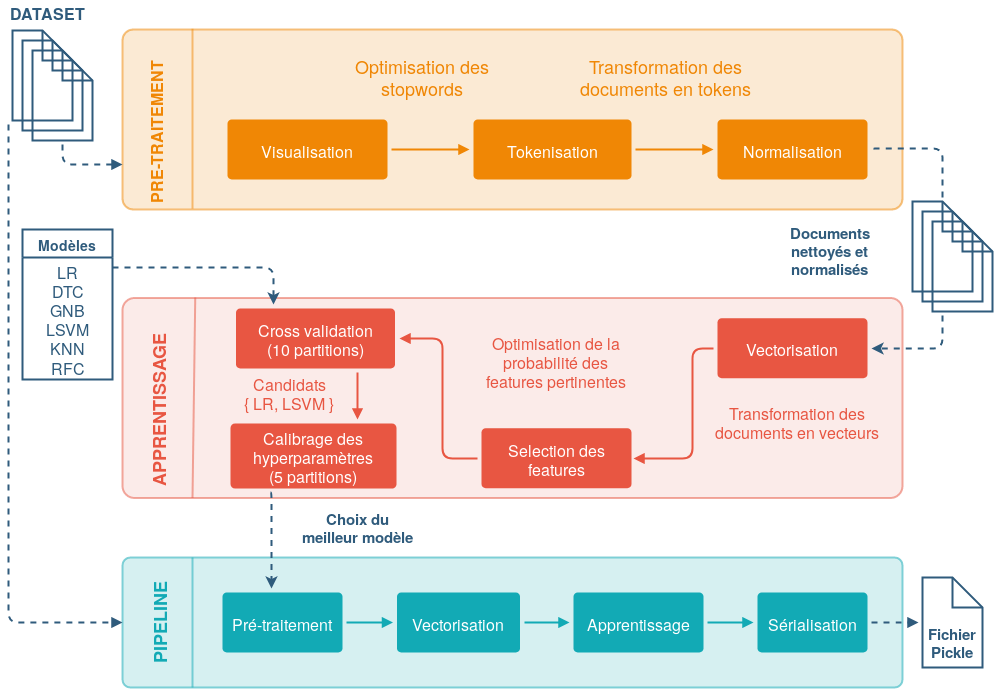
\includegraphics[scale=0.25]{images/conclusion.png}
    \label{fig:global}
\end{figure}
\end{frame}

\end{document}
